% Figure: Treatment Priority — Causal Importance vs Therapeutic Tractability

\begin{figure}[htbp]
\centering
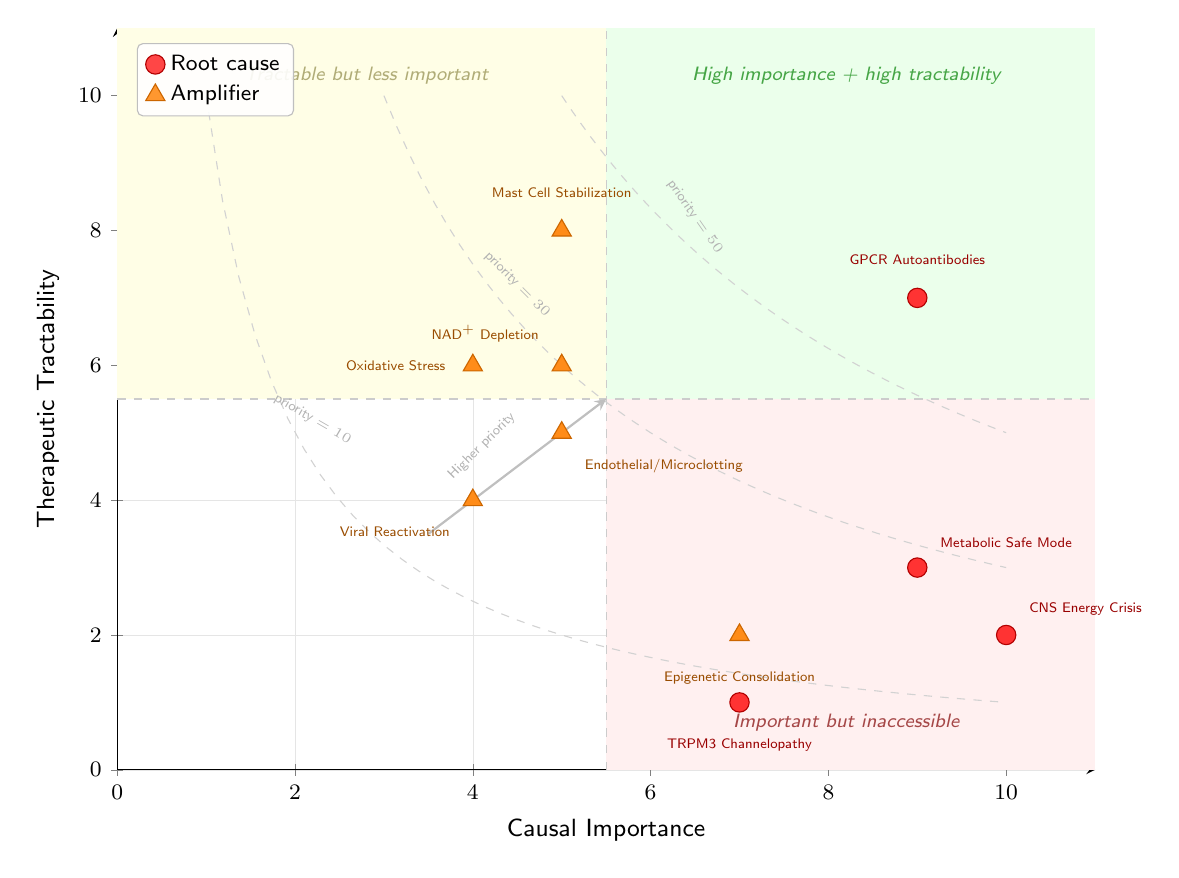
\begin{tikzpicture}[font=\sffamily]
\begin{axis}[
    width=14cm,
    height=11cm,
    xlabel={Causal Importance},
    ylabel={Therapeutic Tractability},
    xmin=0, xmax=11,
    ymin=0, ymax=11,
    xtick={0,2,4,6,8,10},
    ytick={0,2,4,6,8,10},
    grid=major,
    grid style={gray!20, very thin},
    axis lines=left,
    every axis label/.style={font=\sffamily\small},
    every tick label/.style={font=\sffamily\footnotesize},
    clip=false,
    legend style={
        at={(0.02,0.98)},
        anchor=north west,
        font=\sffamily\footnotesize,
        draw=gray!50,
        fill=white,
        fill opacity=0.9,
        text opacity=1,
        cells={anchor=west},
        rounded corners=2pt,
    },
    legend cell align={left},
]

% --- Quadrant shading ---
% Upper-right: sweet spot (green)
\fill[green!8] (axis cs:5.5,5.5) rectangle (axis cs:11,11);
% Lower-right: important but inaccessible (red)
\fill[red!6] (axis cs:5.5,0) rectangle (axis cs:11,5.5);
% Upper-left: tractable but less important (yellow)
\fill[yellow!10] (axis cs:0,5.5) rectangle (axis cs:5.5,11);

% Quadrant dividers
\draw[gray!40, dashed, thin] (axis cs:5.5,0) -- (axis cs:5.5,11);
\draw[gray!40, dashed, thin] (axis cs:0,5.5) -- (axis cs:11,5.5);

% Quadrant labels
\node[font=\sffamily\scriptsize\itshape, text=green!50!black, rotate=0, opacity=0.7]
    at (axis cs:8.2,10.3) {High importance + high tractability};
\node[font=\sffamily\scriptsize\itshape, text=red!50!black, rotate=0, opacity=0.7]
    at (axis cs:8.2,0.7) {Important but inaccessible};
\node[font=\sffamily\scriptsize\itshape, text=yellow!50!black, rotate=0, opacity=0.7]
    at (axis cs:2.8,10.3) {Tractable but less important};

% --- Iso-priority contour lines (priority = importance x tractability) ---
% priority = 10
\draw[gray!35, dashed, thin]
    plot[domain=1:10, samples=50] (\x, {10/\x});
\node[font=\sffamily\tiny, text=gray!60, rotate=-30]
    at (axis cs:2.2,5.2) {priority $= 10$};

% priority = 30
\draw[gray!35, dashed, thin]
    plot[domain=3:10, samples=50] (\x, {30/\x});
\node[font=\sffamily\tiny, text=gray!60, rotate=-45]
    at (axis cs:4.5,7.2) {priority $= 30$};

% priority = 50
\draw[gray!35, dashed, thin]
    plot[domain=5:10, samples=50] (\x, {50/\x});
\node[font=\sffamily\tiny, text=gray!60, rotate=-55]
    at (axis cs:6.5,8.2) {priority $= 50$};

% Arrow indicating direction of higher priority
\draw[-stealth, gray!50, thick] (axis cs:3.5,3.5) -- (axis cs:5.5,5.5);
\node[font=\sffamily\tiny, text=gray!60, rotate=45]
    at (axis cs:4.1,4.8) {Higher priority};

% === ROOT CAUSES (red filled circles) ===
\addplot[
    only marks,
    mark=*,
    mark size=3.5pt,
    color=red!70!black,
    fill=red!80,
] coordinates {
    (10, 2)   % CNS Energy Crisis
    (9, 3)    % Metabolic Safe Mode
    (9, 7)    % GPCR Autoantibodies
    (7, 1)    % TRPM3 Channelopathy
};
\addlegendentry{Root cause}

% === AMPLIFIERS (orange filled triangles) ===
\addplot[
    only marks,
    mark=triangle*,
    mark size=4pt,
    color=orange!80!black,
    fill=orange!90,
] coordinates {
    (5, 6)    % NAD+ Depletion
    (4, 6)    % Oxidative Stress
    (5, 8)    % Mast Cell-Energy Loop
    (4, 4)    % Viral Reactivation
    (5, 5)    % Endothelial/Microclotting
    (7, 2)    % Epigenetic Consolidation
};
\addlegendentry{Amplifier}

% === DATA POINT LABELS ===
% Root causes
\node[font=\sffamily\tiny, anchor=south west, text=red!60!black]
    at (axis cs:10.15,2.15) {CNS Energy Crisis};
\node[font=\sffamily\tiny, anchor=south west, text=red!60!black]
    at (axis cs:9.15,3.15) {Metabolic Safe Mode};
\node[font=\sffamily\tiny, anchor=south, text=red!60!black]
    at (axis cs:9,7.35) {GPCR Autoantibodies};
\node[font=\sffamily\tiny, anchor=north, text=red!60!black]
    at (axis cs:7,0.6) {TRPM3 Channelopathy};

% Amplifiers
\node[font=\sffamily\tiny, anchor=south east, text=orange!60!black]
    at (axis cs:4.85,6.2) {NAD\textsuperscript{+} Depletion};
\node[font=\sffamily\tiny, anchor=east, text=orange!60!black]
    at (axis cs:3.8,6) {Oxidative Stress};
\node[font=\sffamily\tiny, anchor=south, text=orange!60!black]
    at (axis cs:5,8.35) {Mast Cell Stabilization};
\node[font=\sffamily\tiny, anchor=north east, text=orange!60!black]
    at (axis cs:3.85,3.75) {Viral Reactivation};
\node[font=\sffamily\tiny, anchor=north west, text=orange!60!black]
    at (axis cs:5.15,4.75) {Endothelial/Microclotting};
\node[font=\sffamily\tiny, anchor=north, text=orange!60!black]
    at (axis cs:7,1.6) {Epigenetic Consolidation};

\end{axis}
\end{tikzpicture}
\caption{Treatment priority as a function of causal importance and therapeutic tractability.
Mechanisms in the upper-right quadrant (high importance, high tractability) have the highest
treatment priority. The GPCR autoantibody cascade occupies the most favorable position among
root causes; mast cell stabilization is the most favorable amplifier target. Diagonal lines
represent iso-priority contours (Section~\ref{sec:treatment-vs-cause}).}
\label{fig:treatment-priority-scatter}
\end{figure}
